%%% PyKEEN hierarchical extensions overview — COMPACT variant of pykeen_overview.tex.
%%% Same four columns mirroring the paper's paragraph headings, in pipeline order
%%% (Datasets & Analytics -> Evaluation Tasks -> Embedding Models -> Link Prediction
%%% Metrics), wide-and-flat aspect. Per-column "pykeen/ours" group labels are dropped
%%% (colour + legend carry that); the legend sits in a thin strip below the panels.
\documentclass[tikz,border=0pt]{standalone}
\usepackage{amsmath,amssymb}
\usepackage[T1]{fontenc}
\usetikzlibrary{arrows.meta, positioning, shapes.misc, calc, backgrounds, fit}

% ── Colour palette (project-wide) ───────────────────────────────────────
\definecolor{varblue}{HTML}{3B82F6}
\definecolor{edgegray}{HTML}{475569}
\definecolor{titledark}{HTML}{1E293B}
\definecolor{levelbox}{HTML}{94A3B8}
\definecolor{blankslate}{HTML}{64748B}
\definecolor{panelbg}{HTML}{F8FAFC}
\definecolor{querybg}{HTML}{F1F5F9}

\begin{document}
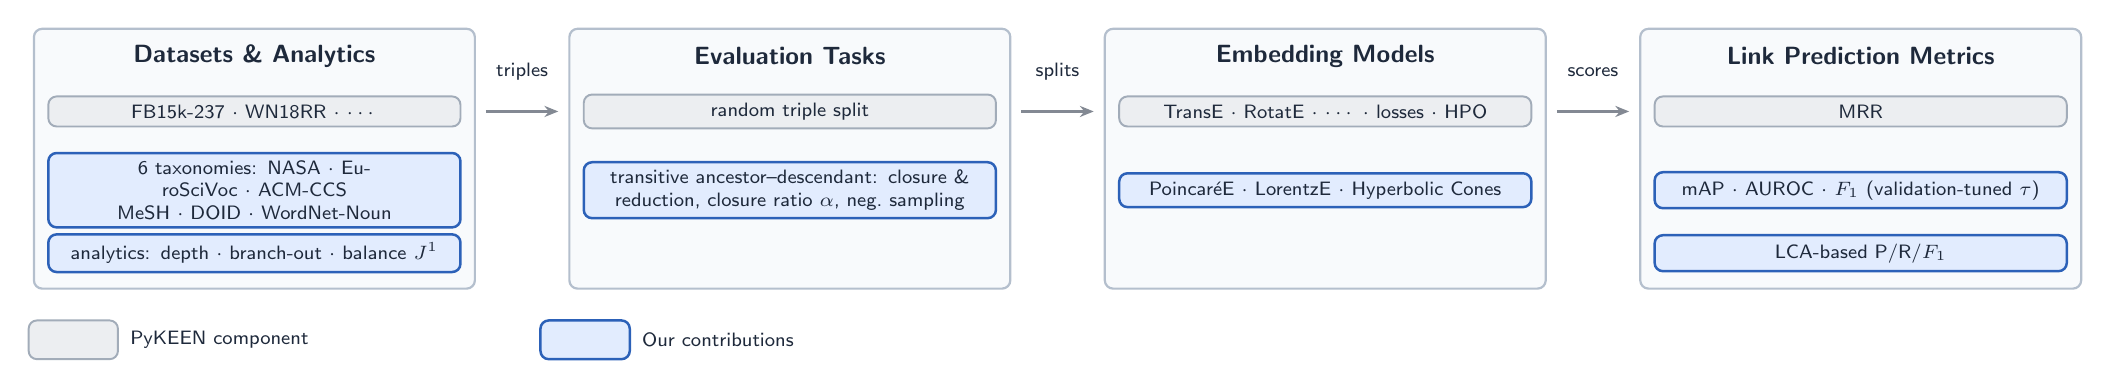
\begin{tikzpicture}[
    font=\sffamily,
    >={Stealth[length=5pt, width=4pt]},
    sub label/.style={font=\scriptsize\sffamily, text=titledark},
    inner box/.style={draw=levelbox!70, line width=0.8pt, rounded corners=3pt,
        fill=panelbg},
    module title/.style={font=\small\sffamily\bfseries\scshape, text=titledark},
    pyk chip/.style={draw=blankslate!60, fill=blankslate!12, rounded corners=3pt,
        line width=0.7pt, font=\scriptsize\sffamily, text=titledark,
        align=center, inner ysep=3pt, text width=#1},
    hp chip/.style={draw=varblue!75!black, fill=varblue!15, rounded corners=3pt,
        line width=0.9pt, font=\scriptsize\sffamily, text=titledark,
        align=center, inner ysep=3pt, text width=#1},
    future chip/.style={draw=varblue!60, dash pattern=on 3pt off 2pt,
        rounded corners=3pt, line width=0.9pt, font=\scriptsize\sffamily,
        text=titledark, align=center, inner ysep=3pt, text width=#1},
    transition/.style={draw=titledark!55, line width=1.4pt, ->,
        shorten <=4pt, shorten >=4pt},
    tlabel/.style={font=\scriptsize\sffamily, text=titledark, align=center},
]

% ══════════════════════════════════════════════════════════════════════
%  DIMENSIONS — four columns on one flat row, uniform chip grid
% ══════════════════════════════════════════════════════════════════════
\def\panelT{0}    \def\panelB{-3.3}
\def\rowA{-1.05}  \def\rowB{-2.05}  \def\rowC{-2.85}   % chip row centres
\def\DL{0}    \def\DR{5.6}    \def\Dcx{2.8}
\def\PL{6.8}  \def\PR{12.4}   \def\Pcx{9.6}
\def\LL{13.6} \def\LR{19.2}   \def\Lcx{16.4}
\def\EL{20.4} \def\ER{26.0}   \def\Ecx{23.2}
\def\chipW{5.0cm}

\begin{scope}[on background layer]
  \draw[inner box] (\DL,\panelB) rectangle (\DR,\panelT);
  \draw[inner box] (\PL,\panelB) rectangle (\PR,\panelT);
  \draw[inner box] (\LL,\panelB) rectangle (\LR,\panelT);
  \draw[inner box] (\EL,\panelB) rectangle (\ER,\panelT);
\end{scope}

\node[module title] at (\Dcx,-0.35) {Datasets \& Analytics};
\node[module title] at (\Pcx,-0.35) {Evaluation Tasks};
\node[module title] at (\Lcx,-0.35) {Embedding Models};
\node[module title] at (\Ecx,-0.35) {Link Prediction Metrics};

% ── Datasets & Analytics ──────────────────────────────────────────────
\node[pyk chip=\chipW] at (\Dcx,\rowA) {FB15k-237 $\cdot$ WN18RR $\cdot$ $\cdots$};
\node[hp chip=\chipW]  at (\Dcx,\rowB)
    {6 taxonomies: NASA $\cdot$ EuroSciVoc $\cdot$ ACM-CCS\\MeSH $\cdot$ DOID $\cdot$ WordNet-Noun};
\node[hp chip=\chipW]  at (\Dcx,\rowC)
    {analytics: depth $\cdot$ branch-out $\cdot$ balance $J^1$};

% ── Evaluation Tasks ──────────────────────────────────────────────────
\node[pyk chip=\chipW] at (\Pcx,\rowA) {random triple split};
\node[hp chip=\chipW]  at (\Pcx,\rowB)
    {transitive ancestor--descendant: closure \&\\reduction, closure ratio $\alpha$, neg.\ sampling};

% ── Embedding Models ──────────────────────────────────────────────────
\node[pyk chip=\chipW] at (\Lcx,\rowA)
    {TransE $\cdot$ RotatE $\cdot$ $\cdots$ $\cdot$ losses $\cdot$ HPO};
\node[hp chip=\chipW]  at (\Lcx,\rowB)
    {Poincar\'eE $\cdot$ LorentzE $\cdot$ Hyperbolic Cones};

% ── Link Prediction Metrics ───────────────────────────────────────────
\node[pyk chip=\chipW] at (\Ecx,\rowA) {MRR};
\node[hp chip=\chipW]  at (\Ecx,\rowB)
    {mAP $\cdot$ AUROC $\cdot$ $F_1$ (validation-tuned $\tau$)};
\node[hp chip=\chipW]  at (\Ecx,\rowC) {LCA-based P/R/$F_1$};

% ── Flow arrows  (data -> task -> model -> metric) ────────────────────
\draw[transition] (\DR,\rowA) -- (\PL,\rowA);
\node[tlabel] at ({(\DR+\PL)/2},-0.55) {triples};
\draw[transition] (\PR,\rowA) -- (\LL,\rowA);
\node[tlabel] at ({(\PR+\LL)/2},-0.55) {splits};
\draw[transition] (\LR,\rowA) -- (\EL,\rowA);
\node[tlabel] at ({(\LR+\EL)/2},-0.55) {scores};

% ══════════════════════════════════════════════════════════════════════
%  LEGEND — thin strip below the panels
% ══════════════════════════════════════════════════════════════════════
\node[pyk chip=0.9cm] at (0.5,-3.95) {\strut};
\node[sub label, anchor=west] at (1.1,-3.95) {PyKEEN component};
\node[hp chip=0.9cm] at (7.0,-3.95) {\strut};
\node[sub label, anchor=west] at (7.6,-3.95) {Our contributions};

\end{tikzpicture}
\end{document}
